\apendice{Especificación de diseño}

\section{Introducción}
En esta sección se va a explicar como se ha diseñado la aplicación para que realice los objetivos y requisitos de la misma. También se mostrarán los diagramas correspondientes, aunque se han simplificado omitiendo algunos elementos como los atributos o métodos para mejorar su representación.

\section{Diseño de datos}
La aplicación se divide en dos grandes bloques. Por una parte están los algoritmos que planifican la ruta y por otra están las clases que se dedican a realizar tareas con las rutas que devuelven los algoritmos.

La clase MoverCoche es la clase principal y se encarga de seleccionar el algoritmo, recoger la ruta y proporcionarsela en orden a las clases de suavizado, PathSmoothing y de movimiento, PIDControl.

También se encarga de instanciar e iniciar las clases auxiliares y parámetros necesarios, y es desde MoverCoche donde se sigue el bucle continuo del motor gráfico para realizar las operaciones.

\begin{figure}[htpb]
    \centering
    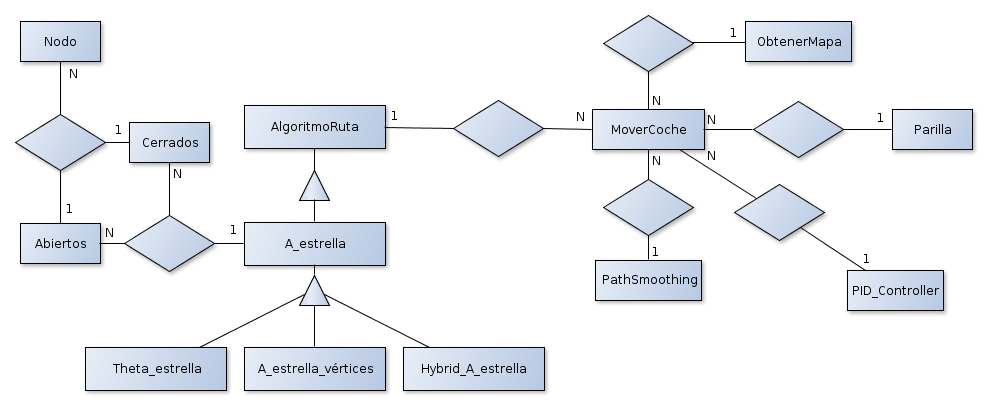
\includegraphics[width=\textwidth,height=10cm,keepaspectratio=true]{c_entidad_relacion}
    \caption[Diagrama entidad relación]{Diagrama entidad relación.}
    \label{fig:centidadrelacion}
\end{figure}

\section{Diseño procedimental}
\textit{Unity} como motor gráfico forma parte de la aplicación. La forma de usar \textit{Unity} es a través de \textit{scripts} que heredan de la clase \textit{MonoBehaviour} y enlazandoles con algún elemento de la escena que hayamos creado.

Por ejemplo, en nuestro proyecto, tanto la clase de MoverCoche como la de AlgoritmosRuta heredan de \textit{MonoBehaviour}, de tal forma que les podemos enlazar con el \textit{GameObject} que creamos con el editor para el coche.

Estas clases tienen varios métodos que permiten ser usados cuando se inicia la ejecución, y desde ese punto llamar al resto de clases y métodos. Para este proyecto hemos usado los métodos \textit{Start()}, \textit{FixedUpdate()} y \textit{Update()}.
\begin{itemize}
\item \textbf{\textit{Start()}}: este método se ejecuta cuando se cargue en la escena el objeto al que esta enlazado. Se utiliza para la inicialización de elementos.
\item \textbf{\textit{FixedUpdate()}}: este método se ejecuta a intervalos de tiempo cortos (más rápido que un \textit{frame}), y se utiliza para el cálculo de las físicas.
\item \textbf{\textit{Update()}}: este método se ejecuta cada \textit{frame}, y se utiliza para toda la lógica que no involucre a las físicas.
\end{itemize}

El vehículo se carga al inicio de la ejecución puesto que está presente en la escena que hemos creado, y por tanto el primer método que se ejecutará será el \textit{Start()} de MoverCoche que tiene enlazado. Se usa para iniciar todo lo necesario para realizar tanto la ejecución de los algoritmos de búsqueda de rutas, como las clases que hacen uso de la ruta como \textit{PathSmoothing} y \textit{PIDControl}. Es aquí también donde dependiendo de las opciones seleccionados se elegirá un algoritmo u otro para el cálculo de la ruta.

A continuación el programa se ejecuta como un bucle continuo donde se están constantemente llamando a \textit{Update()} y \textit{FixedUpdate()}. Se ha usado \textit{Update()} para realizar la búsqueda de la ruta, de tal forma que cada llamada a \textit{Update()} corresponde con un ciclo del algoritmo correspondiente. En cada una de esas llamadas también se dibujan el progreso del algoritmo en su búsqueda. \textit{FixedUpdate()} no se utiliza hasta que se ha obtenido una ruta. Al ser usado para el cálculo de las físicas, y por tanto de la simulación del vehículo y su movimiento, hasta que no haya una ruta que seguir no se hace uso de él. Cuando ya se ha obtenido una ruta, se deja de usar \textit{Update()}, y se pasa a mover el vehículo desde \textit{FixedUpdate()}.

\begin{figure}[htpb]
    \centering
    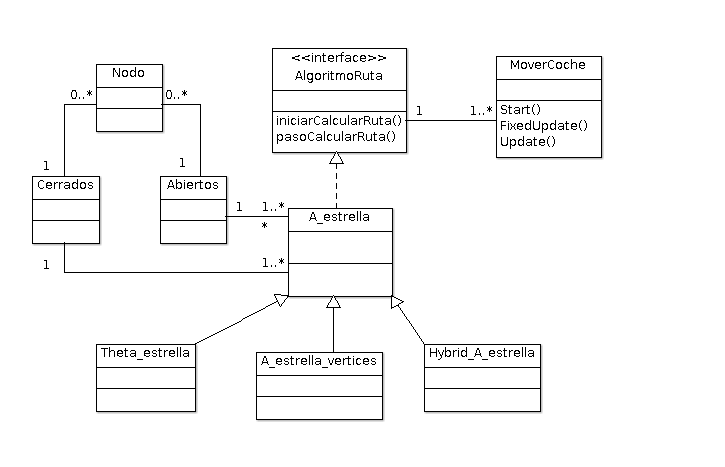
\includegraphics[width=\textwidth,height=10cm,keepaspectratio=true]{c_clases_algoritmos}
    \caption[Diagrama de clases de los algoritmos]{Diagrama de clases de los algoritmos.}
    \label{fig:cclasesalgoritmos}
\end{figure}

Se ha creado la interfaz AlgoritmoRuta para que en el futuro, implementando los métodos de la interfaz, se puede enlazar y/o instanciar en MoverCoche con lo que facilite la creación de algoritmos nuevos. En el caso de los algoritmos que se han implementado, son el A* o algoritmos que modifican el A*, por lo que hemos se ha usado el A* y se han ido modficando en las subclases los métodos que fueran necesarios.

\begin{figure}[htpb]
    \centering
    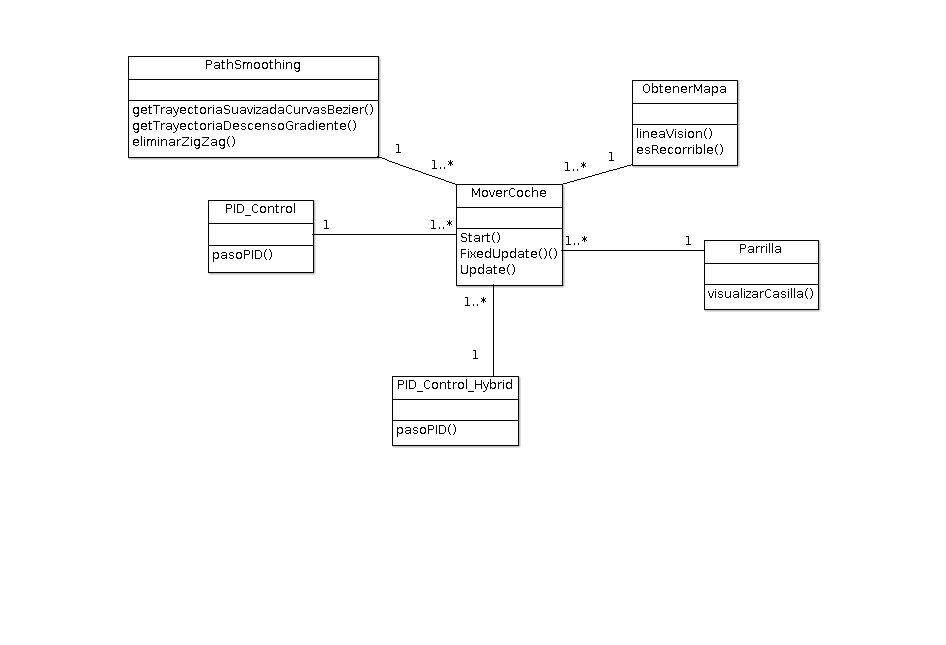
\includegraphics[width=\textwidth,height=10cm,keepaspectratio=true]{c_clases_rutas}
    \caption[Diagrama de clases del manejo de las rutas]{Diagrama de clases del manejo de las rutas.}
    \label{fig:cclasesrutas}
\end{figure}

Una vez obtenida la ruta, se pasa a la siguiente fase de la ejecución. En primer lugar se suaviza la ruta con los métodos de PathSmoothing, y a continuación se realiza el movimiento del vehículo. Para el movimiento se realiza desde \textit{FixedUpdate()}, como comentamos anteriormente, y de igual manera se realiza paso a paso en cada una de sus ejecuciones. Para le movimiento autónomo, se llama en cada ejecución a \textit{PIDControl} pata que actualice los valores necesarios para el motor y las ruedas teniendo en cuenta el desplazamiento que ha ocurrido desde la anterior iteración.

\section{Diseño arquitectónico}
En la figura \ref{fig:cdiagramasecuencia} podemos observar como se relacionan todas las clases principales a partir de MoverCoche.

Las dos primeras llamadas, iniciarCalcularRuta() y getMapaDistancias(), se ejecutan en el método \textit{Start()} fuera del bucle continuo del motor gráfico. Con iniciarCalcularRuta() se prepara para iniciarse el algoritmo, creando todos los elementos que necesite. En este ejemplo obtenemos el mapa de distancias puesto que se crea al iniciarse el \textit{Hybrid A*} ya que lo necesita durante su ejecución.

A continuación, se  realiza la llamada a pasoCalcularRuta() que se ejecuta en \textit{Update()}, formando ya parte del bucle continuo. Al ser \textit{Update()}, se ejecutan una vez por cada frame. Es aquí donde se realiza la búsqueda de la ruta por parte del algoritmo y dibuja el progreso de su ejecución. Cuando termina la búsqueda, en ese ciclo se llama a getTrayectoriaDescensoGradiente() para suavizar el resultado.

Y por último, la llamada a pasoPID() se realiza en \textit{FixedUpdate()}, que se ejecuta a un intervalo fijo de tiempo, más rápido que a cada \textit{frame}. Como es el método destinado al cálculo de las físicas, se realiza la llamada a pasoPID() para obtener los valores de la fuerza del motor y del giro de las ruedas para que el vehículo se mueva de una forma autónoma.

\begin{figure}[htpb]
    \centering
    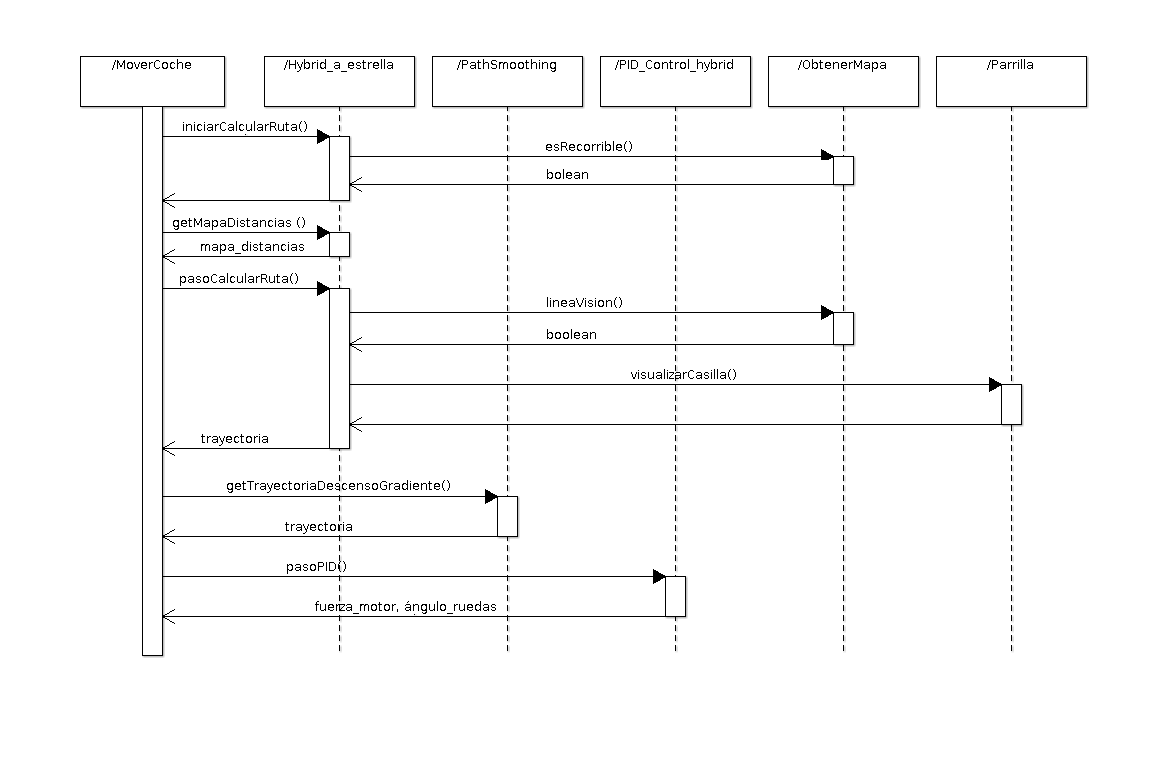
\includegraphics[width=\textwidth,height=20cm,keepaspectratio=true]{c_diagrama_secuencia}
    \caption[Diagrama de secuencia]{Diagrama de secuencia usando el algoritmo \textit{Hybrid A*}.}
    \label{fig:cdiagramasecuencia}
\end{figure}


